% sections/problem2.tex

\subsection{问题分析与模型构建：负荷与光伏预测不确定性下的日前购电调度}\label{subsec:q2-analysis}
问题一基于典型日完全信息得到确定性调度基准；问题二将模型拓展至全年连续仿真，只允许每日0:00利用当前信息签订全天日前购电合同，合同签订后日内不可调整。若出现功率缺口，缺口部分按5倍电价应急购电。本问题的核心权衡是：合同电量偏低会触发高额应急购电成本，合同过量则产生无法退回的闲置合同费用。

本文对问题二的处理分为五个环节：先比较两组只使用历史数据的点预测方案并确定预测器；再对同一预测版本下的净负荷残差作逐时段经验分位修正，得到安全轨迹；随后以安全轨迹、真实日初储电量与分时电价求解0:00日前合同线性规划；日内以预测驱动的滚动时域线性规划（MPC执行器）执行储能动作；最后代入真实负荷与光伏完成裁剪、平衡与结算。技术流程如图\ref{fig:q2_flow}所示。

\begin{figure}[htbp]
\centering
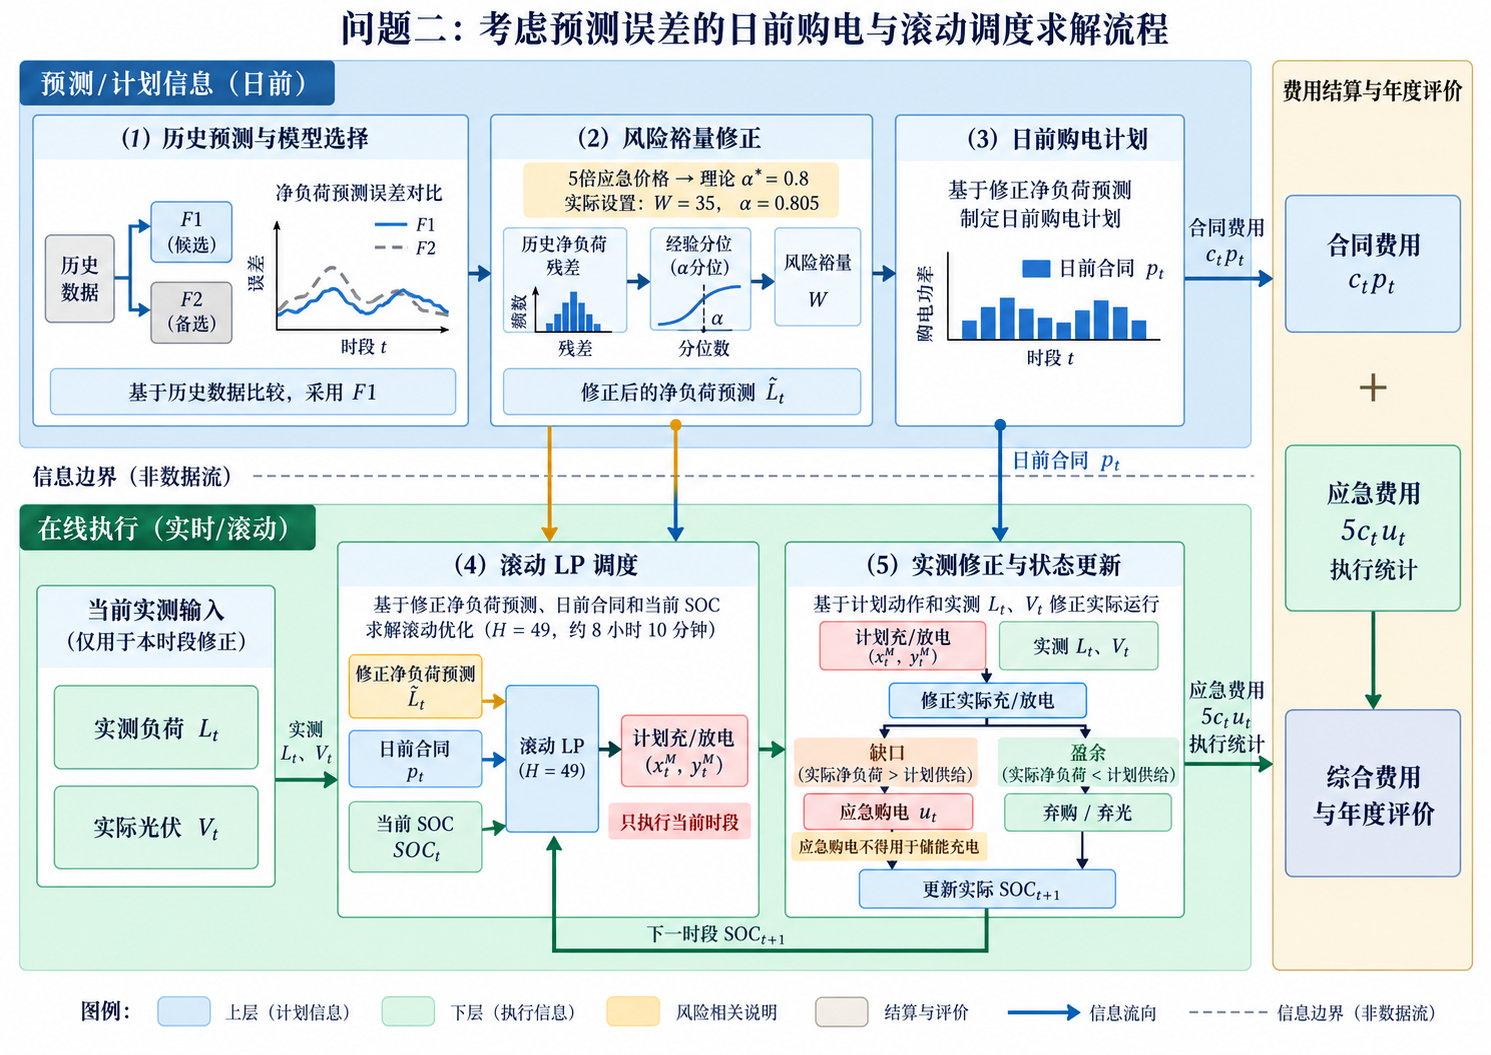
\includegraphics[width=0.90\textwidth]{figures/q2-flow.png}
\caption{问题二预测驱动日前购电与MPC执行流程}
\label{fig:q2_flow}
\end{figure}

\subsection{历史预测方案对比与选型依据}\label{subsec:q2-forecast}
本文比较两种只使用目标日前历史观测的负荷与光伏预测方法，记目标日为$d$、时段为$t$。负荷和光伏预测的常用方法及误差来源可参考相关综述\cite{hong2020forecasting,iheanetu2022pvforecasting}。F1为主预测器：负荷采用一周前同一时段的观测值，光伏采用前七日同一时段的均值，分别为
\begin{align}
\widehat L^{F1}_{d,t} &= L_{d-7,t}, \label{eq:q2-f1l}\\
\widehat V^{F1}_{d,t} &= \frac{1}{7}\sum_{k=1}^{7}V_{d-k,t}. \label{eq:q2-f1v}
\end{align}
F2仅将负荷改为前三个滞后周同一时段观测值的中位数，以减弱单周异常影响；光伏预测与F1相同：
\begin{equation}
\widehat L^{F2}_{d,t}=\operatorname{median}\left(L_{d-7,t},L_{d-14,t},L_{d-21,t}\right).
\label{eq:q2-f2l}
\end{equation}
历史样本不足时按实际可用数据构造预测；1月初无法取得完整滞后样本时的降级处理，统一按第\ref{subsec:data-preprocess}节的规则执行。

点预测精度用平均绝对误差与均方根误差衡量：
\begin{equation}
\mathrm{MAE}=\frac{1}{n}\sum_{i=1}^{n}\left|z_i-\widehat z_i\right|,\qquad
\mathrm{RMSE}=\sqrt{\frac{1}{n}\sum_{i=1}^{n}\left(z_i-\widehat z_i\right)^2}.
\label{eq:q2-metrics}
\end{equation}
两种预测方案在2025年2月1日至12月31日上的误差如表\ref{tab:q2_forecast_error}所示。

\begin{table}[htbp]
\centering
\caption{历史预测方案的误差对比}
\label{tab:q2_forecast_error}
\small
\begin{tabular}{lrrrr}
\toprule
预测器 & 负荷MAE & 光伏MAE & 净负荷MAE & 净负荷RMSE \\
\midrule
F1 & 176.80 & 153.40 & 273.35 & 389.97 \\
F2 & 187.90 & 153.40 & 284.35 & 403.25 \\
\bottomrule
\multicolumn{5}{c}{单位：kW。}\\
\end{tabular}
\end{table}

由表\ref{tab:q2_forecast_error}可得，F1的净负荷MAE与RMSE均低于F2；二者光伏预测完全一致，因此差异可归因于负荷预测方法。基于上述误差及第\ref{subsec:q2-result}节统一执行、结算口径下的闭环费用，本文选取F1为主预测器。


\subsection{净负荷残差的经验分位风险修正}\label{subsec:q2-risk}
记中心净负荷预测为$\widehat N_{d,t}=\widehat L_{d,t}-\widehat V_{d,t}$，同一预测版本下已完成日$j<d$的逐时段残差定义为
\begin{equation}
e^N_{j,t}=N_{j,t}-\widehat N_{j,t},\qquad j<d .
\label{eq:q2-resid}
\end{equation}
使用目标日之前最近$W$个已完成日的同一时段残差经验分位构造安全净负荷：
\begin{equation}
\widetilde N_{d,t}=\widehat N_{d,t}+Q_\alpha\left\{e^N_{j,t}:\ d-W\le j<d\right\}.
\label{eq:q2-safe}
\end{equation}
式\eqref{eq:q2-safe}直接对残差的经验分布取分位，不要求残差服从正态分布，也不需要额外的场景生成步骤；$W$控制所使用历史误差的时间范围，$\alpha$控制风险裕度的位置。加入分位裕度后净负荷可能出现负值，为保持重构后的负荷与光伏非负，按
\begin{equation}
\widetilde V_{d,t}=\max\left(\widehat V_{d,t},-\widetilde N_{d,t},0\right),\qquad
\widetilde L_{d,t}=\widetilde V_{d,t}+\widetilde N_{d,t}
\label{eq:q2-reconstruct}
\end{equation}
将其重新表示为非负的负荷预测与光伏预测。该处理只改变净负荷的分解方式，不改变$\widetilde N_{d,t}$本身，因而不影响供需缺口的计算。

分位水平$\alpha$由计划电价与应急购电价格的比值确定。考虑单个时段，计划购电价格为$c>0$、计划购电量为$p$，该时段净负荷$N$为随机变量，剩余缺口按$5c$应急购电，则该时段的期望费用为
\begin{equation}
J(p)=cp+5c\,\mathbb E\left[(N-p)^+\right],\qquad (N-p)^+=\max(N-p,0).
\label{eq:q2-newsboy}
\end{equation}

\noindent\textbf{命题 2（5倍应急价格对应的报童临界分位）}　在合同单位成本为$c>0$、缺电应急购电单价为$5c$、富余合同不退款的条件下，使式\eqref{eq:q2-newsboy}最小的计划购电量为$N$的$0.8$分位，即$p^*=Q_{0.8}(N)$。

\noindent\textbf{证明}　记$N$的分布函数为$F(\cdot)$。对式\eqref{eq:q2-newsboy}关于$p$求导，
\[
J'(p)=c-5c\,\mathbb P(N>p)=c\left[1-5\left(1-F(p)\right)\right].
\]
令$J'(p)=0$得$F(p)=1-c/(5c)=0.8$，即$p^*=Q_{0.8}(N)$。再对$J'(p)$求导得$J''(p)=5c\,f(p)\ge0$，故$J(p)$为凸函数，该驻点即全局最小值点；$N$取离散分布时按次梯度理解，结论不变。证毕。

命题2的边际含义是：多购1 kWh计划电需支付$c$，少购1 kWh计划电则以$1-\alpha$的概率支付$5c$，两种边际代价相等时分位水平为$1-1/5=0.8$。实际计算中净负荷的分布未知，本文用最近$W=35$个已完成日的同一时段历史残差经验分位数实现该分位水平；受有限样本影响，分位取值与理论值存在小幅差别，主配置取$\alpha=0.805$。该分位仅表示单时段风险基准：命题2针对单个时段的边际分布，$0.8$并不表示整日供电可靠度为$80\%$，也不保证计入储能跨时段耦合后合同量随分位单调变化，因此$W$与$\alpha$的最终取值由第\ref{subsec:q2-result}节的参数敏感性确定。以夏至日为例，分位风险修正前后的净负荷预测与实际净负荷对比如图\ref{fig:q2-safe}所示。

\begin{figure}[htbp]
\centering

\includegraphics[width=0.80\textwidth]{figures/q2-safe.png}
\caption{分位风险修正预测、风险裕量与实际净负荷（以2025-06-21为例）}
\label{fig:q2-safe}
\end{figure}

\subsection{日前合同优化与MPC滚动执行规则}\label{subsec:q2-model}
每天0:00以真实日初储电量为初值、以安全轨迹为输入求解日前合同。规划层令生效合同量$g_t=p_t$，并沿用前文的能量平衡、储能递推和设备边界约束：
\begin{equation}
\min\ \sum_{t=1}^{144}c_tp_t-\lambda\left(S^{P}_{145}-S_{\min}\right),
\label{eq:q2-contract}
\end{equation}
式\eqref{eq:q2-contract}的第一项表示日前合同费用；第二项为有限时域末储能状态设置的机会价值，用于减轻优化时域截断造成的过度放空，$\lambda$仅用于引导求解，不计入实际现金费用。规划层不设置可自由替代的应急购电变量，风险只通过安全轨迹进入合同决策，5倍应急电价在真实执行和结算阶段体现。

问题二按日结算的实际现金费用为
\begin{equation}
C_2=\sum_{t=1}^{144}\left(c_tp_t+5c_tu_t\right).
\label{eq:q2-cash}
\end{equation}
计划购电量无论是否全部消纳均按合同计费，弃购成本已包含在$c_tp_t$中；$5c_tu_t$仅在真实执行出现供电缺口时产生。全年334天闭环仿真中，将各日的$C_2$累加得到现金总费用\textbf{14786101.35元}，其中计划购电费用为\textbf{13665855.74元}，应急购电费用为\textbf{1120245.61元}。由于题目未设并网功率上限，若在日前规划中加入可自由替代的应急变量，模型会倾向于以应急购电替代合同购电，从而失去风险合同规划的含义。因此，本文将合同规划与真实闭环结算分开处理。

合同签订后日内不可调整，储能动作由预测驱动的滚动时域线性规划（MPC执行器，下文简称滚动LP）给出。合同费用在签订时已经确定，因此滚动LP只优化预测的应急购电费用、储能终端价值和极小充放电总量惩罚。在时段$t$，滚动LP以$\mathcal H_t=\{t,\dots,\min(t+H-1,144)\}$为范围，取$H=49$（约8小时10分钟），在$I_{d,t}$给定的信息下安排充放电、光伏利用、弃购、应急购电与储电量：
\begin{equation}
\min\ \sum_{\tau\in\mathcal H_t}5\widehat c_\tau u_\tau
+\varepsilon\sum_{\tau\in\mathcal H_t}\left(x_\tau+y_\tau\right)-\lambda S_{\mathrm{end}},
\label{eq:q2-rolling-obj}
\end{equation}
其中约束为通用能量平衡、储能递推与设备运行边界，$\widehat c_\tau$为当前可用的电价预测。每次求解只执行当前时段动作，下一时段再用更新后的真实储电量重新计算；$\varepsilon$为极小罚项，用于在多重最优解中抑制同时充放电的数值伪解。

由于执行层的合同费用已经确定，命题1关于规划层自由购电变量的结论不能直接套用。对执行层，$\varepsilon(x_\tau+y_\tau)$用于选取无同时充放电的数值解，并有如下条件性说明。

\noindent\textbf{命题 3（滚动执行层的储能互斥性，附条件）}　考虑窗口$\mathcal H_t$内任一时段$\tau$的滚动LP（式\eqref{eq:q2-rolling-obj}）及其功率平衡、SOC递推约束。若某最优解在$\tau$处满足$x_\tau>0,y_\tau>0$，且下列两个条件至少有一个成立，则与最优性矛盾：
\begin{enumerate}[label=(\Alph*)]
    \item 当期存在吸收余量：$w_\tau<g_\tau$，或$v_\tau>0$（此时$V_\tau>0$），或$u_\tau>0$；
    \item 电池有下游余量：存在$\delta>0$，使从$\tau$到窗口末尾的所有时段，将SOC抬高$\delta(1/\eta_d-\eta_c)$后仍不超过$S_{\max}$。
\end{enumerate}
因此，在上述任一条件下，任一最优解均满足$\min(x_\tau,y_\tau)=0$。

\noindent\textbf{证明}　先取充分小的$\delta>0$，令$x'_\tau=x_\tau-\delta/\eta_c$、$y'_\tau=y_\tau-\delta\eta_d$。由
\[
\eta_cx'_\tau-y'_\tau/\eta_d=\eta_cx_\tau-y_\tau/\eta_d
\]
知$\tau$及其后SOC轨迹不变，$-\lambda S_{\mathrm{end}}$项不受影响。功率平衡左右两侧之差为$\delta(1/\eta_c-\eta_d)>0$，需由$w_\tau,v_\tau,u_\tau$之一吸收；若条件(A)成立，取相应变量吸收该差额后仍可行。若由$w_\tau$或$v_\tau$吸收，应急购电项不变；若由$u_\tau$吸收，该项进一步减少。无论何种情形，$\varepsilon(x_\tau+y_\tau)$项均严格减少$\varepsilon\delta(1/\eta_c+\eta_d)$，目标函数严格改进，与最优性矛盾。

若条件(A)不成立，即$w_\tau=g_\tau,v_\tau=0,u_\tau=0$同时发生，则功率平衡退化为$y_\tau=L_\tau+x_\tau$。取$\delta\leq\min(x_\tau,y_\tau)$，令$x'_\tau=x_\tau-\delta$、$y'_\tau=y_\tau-\delta$，功率平衡两侧同减$\delta$而保持不变，SOC增量变为$\delta(1/\eta_d-\eta_c)>0$；若条件(B)成立则仍可行。此时$\varepsilon(x_\tau+y_\tau)$项减少$2\varepsilon\delta$，且$S_{\mathrm{end}}$增大使$-\lambda S_{\mathrm{end}}$项不增，目标函数同样严格改进，仍与最优性矛盾。证毕。

\noindent\textbf{说明}　当两个条件均不满足时，可能出现外部吸收渠道和电池余量同时受限的特殊边界情形。对此，本文不再引入额外的整数变量或复杂的互斥约束，而是在目标函数中加入极小的充放电总量惩罚项，以较低的建模和求解代价选取无同时充放电的解，同时保持滚动LP的线性结构。第七章的全量求解结果均满足$\min(x_t,y_t)=0$，表明这一简化处理在全年闭环仿真中未造成实际偏差。

设滚动LP给出的当前时隙动作记为$(x_t^M,y_t^M)$。本时隙真实负荷与光伏到达后，只允许在已决定动作的基础上缩减：
\begin{align}
x_t^E&=\min\left\{x_t^M,\ \left(g_t+V_t-L_t\right)^+\right\}, \label{eq:q2-clip-charge}\\
y_t^E&=\min\left\{y_t^M,\ \left(L_t-g_t-V_t+x_t^E\right)^+\right\}, \label{eq:q2-clip-discharge}\\
b_t&=L_t+x_t^E-y_t^E-g_t-V_t. \label{eq:q2-clip-gap}
\end{align}
若$b_t\ge0$，则$u_t=b_t$、$w_t=0$；若$b_t<0$，则$u_t=0$，并将$-b_t$依次解释为未利用合同电量与弃光电量。式\eqref{eq:q2-clip-charge}至式\eqref{eq:q2-clip-gap}保证应急电只补实际缺口、不用于主动充电，同时禁止执行层依据本时隙实测缺口临时增加放电，使两种执行器在同一信息集下可比。时隙末真实储电量由储能递推关系传入下一时隙。

作为同信息集对照，本文另设预测驱动贪心执行器。令预测盈余
\[
A_t=g_t+\widetilde V_{d,t}-\widetilde L_{d,t},
\]
若$A_t\ge0$，则盈余用于充电：
\[
x_t=\min\left\{A_t,\ B_{\max},\ \frac{S_{\max}-S_t^E}{\eta_c}\right\},\qquad y_t=u_t=0;
\]
若$A_t<0$，则先放电、缺口再应急：
\[
y_t=\min\left\{-A_t,\ B_{\max},\ \left(S_t^E-S_{\min}\right)\eta_d\right\},\qquad u_t=-A_t-y_t,\qquad x_t=w_t=0.
\]
贪心只依据当前一个时隙的安全轨迹决定动作，同样在动作确定之后才读取实测值并调用式\eqref{eq:q2-clip-charge}至式\eqref{eq:q2-clip-gap}的统一裁剪器。两种执行器共享同一合同、预测方法、风险裕度、储能约束与结算规则，唯一差别是滚动LP额外利用了未来$H$个时隙的价格与安全轨迹信息。贪心执行器作为同信息集下的可行基线，不代表跨时段最优；年度正式结果以滚动LP为主执行器。

\subsection{年度仿真结果与对比分析}\label{subsec:q2-result}
334天仿真结束后，年度关键指标如表\ref{tab:q2_result_sum}所示。

\begin{table}[htbp]
\centering
\caption{问题二年度运行汇总结果（2--12月）}
\label{tab:q2_result_sum}
\scriptsize
\begin{tabular}{@{}p{0.29\textwidth}r@{\quad}p{0.29\textwidth}r@{}}
\toprule
指标 & 数值 & 指标 & 数值 \\ 
\midrule
计划购电量 & 22382650.65 $\mathrm{kWh}$ & 计划购电费用 & 13665855.74 元 \\ 
应急购电量 & 245483.29 $\mathrm{kWh}$ & 应急购电费用 & 1120245.61 元 \\ 
应急购电发生时段数 & 6822 & 闲置合同电量 & 1596110.94 $\mathrm{kWh}$ \\
弃光电量 & 1741589.34 $\mathrm{kWh}$ & 储能充电量 & 7112133.95 $\mathrm{kWh}$ \\ 
储能放电量 & 5760889.78 $\mathrm{kWh}$ & 期末储电量 & 10731.91 $\mathrm{kWh}$ \\ 
\multicolumn{3}{l}{年度现金总费用} & \textbf{14786101.35 元} \\ 
\bottomrule
\end{tabular}
\end{table}

由表\ref{tab:q2_result_sum}可得，全年计划购电量为\textbf{22382650.65 kWh}，现金总费用为\textbf{14786101.35元}，其中计划购电费用为\textbf{13665855.74元}、应急购电费用为\textbf{1120245.61元}。应急购电量为\textbf{245483.29 kWh}，仅占合同电量的$1.10\%$，但对总费用的贡献达到$7.58\%$，说明风险修正将部分预测误差损失转化为可控的合同冗余。全年弃购\textbf{1596110.94 kWh}、弃光\textbf{1741589.34 kWh}；储能全年充电\textbf{7112133.95 kWh}、放电\textbf{5760889.78 kWh}，期末储电量为\textbf{10731.91 kWh}，全程满足安全边界。按月统计，12月费用最高，6月应急购电量最高，4月费用最低，反映了负荷和光伏的季节性影响。

为检验主配置的稳健性，对预测器、残差窗口、分位水平与滚动时域逐一重跑全年闭环仿真，结果如表\ref{tab:q2_sensitivity}所示。

\begin{table}[htbp]
\centering
\caption{问题二预测器与参数敏感性汇总（2--12月）}
\label{tab:q2_sensitivity}
\scriptsize
\setlength{\tabcolsep}{3.5pt}
\begin{tabular}{llrrr}
\toprule
类别 & 设置 & 年度费用/元 & 应急购电/kWh & 费用变化/元 \\
\midrule
主配置 & F1,$W=35$,$\alpha=0.805$,$H=49$ & 14786101.35 & 245483.29 & 0.00 \\
预测器 & F2 & 14788842.58 & 249032.38 & +2741.23 \\
风险分位 & $\alpha=0.800/0.810$ & 14820043.34/14786818.42 & 289390.70/245477.85 & +33941.99/+717.07 \\
残差窗口 & $W=30/45$ & 14837364.77/14815783.49 & 247334.59/260994.56 & +51263.42/+29682.14 \\
滚动时域 & $H=48/50$ & 14786354.19/14786319.50 & 245523.92/245518.43 & +252.84/+218.15 \\
\bottomrule
\end{tabular}
\end{table}

表\ref{tab:q2_sensitivity}将预测器、风险分位、残差窗口和滚动时域的试验统一列示。各备选配置相对主方案的费用变化不超过$0.35\%$；其中$H$的小幅变化影响最小，F2替换F1仅增加2741.23元，而较低分位和较短残差窗口会明显增加费用。因此采用F1、$W=35$、$\alpha=0.805$和$H=49$作为主配置。

为评价风险修正策略的相对水平，另设两组参照方案开展全周期对照：理想信息参照假设调度日0:00完全已知真实负荷与光伏，仅作为事后不可实施的理论下界；无储能基线为理想净负荷信息下的无储能参照。结果如表\ref{tab:q2_baseline_compare}所示。

\begin{table}[htbp]
\centering
\caption{不同参照方案年度运行指标对比（2--12月）}
\label{tab:q2_baseline_compare}
\scriptsize
\begin{tabular}{lrrr}
\toprule
方案 & 年度现金费用/元 & 应急购电费用/元 & 应急购电量/kWh \\
\midrule
主配置 F1-W35-$\alpha$0.805-H49 & 14786101.35 & 1120245.61 & 245483.29 \\
理想信息参照（事后下界，不可实施） & 12291024.77 & 0.00 & 0.00 \\
无储能基线 & 16407319.63 & 0.00 & 0.00 \\
\bottomrule
\end{tabular}
\end{table}

理想信息参照与主配置的差额2495076.58元，度量了全年负荷与光伏预测不确定性带来的总经济代价。无储能参照仅用于刻画“即使不给储能、但已知当期净负荷”时的参考费用，不用于严格分离储能边际贡献。该参照方案为规避缺口必须按更保守的口径采购合同电量，全年不产生应急购电，但现金费用高出主配置1621218.28元（约$11.0\%$）。该对比说明储能的削峰填谷收益只有在合理预测与风险裕度配合下才能实现：储能本身并不能消除预测误差，它把误差从高价应急购电转移到合同冗余与充放电总量两侧，而这一转移是否盈利取决于分位裕度设置是否合理。

四个代表日的运行结果如表\ref{tab:q2_repday}与图\ref{fig:q2-days}所示。

\begin{table}[htbp]
\centering
\caption{问题二四个代表日（春分、夏至、秋分、冬至）运行结果}
\label{tab:q2_repday}
\scriptsize
\begin{tabular}{lrrrr}
\toprule
日期 & 日购电费用/元 & 计划购电量/kWh & 应急购电量/kWh & 日初--日末储电量/kWh \\
\midrule
2025-03-20 & 45158.05 & 70894.49 & 542.74 & 10800.00--10795.24 \\
2025-06-21 & 24282.59 & 41689.27 & 9.36 & 10800.00--10800.00 \\
2025-09-23 & 47616.38 & 72083.06 & 600.29 & 10760.83--10793.77 \\
2025-12-21 & 66632.03 & 101642.57 & 234.75 & 10756.53--10800.00 \\
\bottomrule
\end{tabular}
\end{table}

\begin{figure}[htbp]
\centering

\includegraphics[width=0.90\textwidth]{figures/q2-days.png}
\caption{春分、夏至、秋分、冬至四个代表日的购电功率与储电量}
\label{fig:q2-days}
\end{figure}

代表日结果与光伏季节性一致：12月21日负荷高、光伏弱，日费用最高（66632.03元）；6月21日光伏充足，日费用最低（24282.59元）；3月20日与9月23日的应急购电分别集中在凌晨与清晨的连续缺口时段，说明应急购电风险与日内负荷、光伏变化密切相关，而非由全天平均工况决定。上述代表日按题目要求整理的指定时段购电量、4小时充放电与储电量、应急购电区间见附录。

最后需要说明风险裕度的工程折中关系：裕度设置过高会抬高合同采购成本并增加弃购，裕度设置过低则应急购电风险上升。仿真会观测到同一日内同时存在闲置合同电量与应急购电的现象，根源在于日前合同按时隙固定，跨时隙合同电量无法调剂；这属于赛题交易规则与逐时段负荷、光伏变化共同造成的客观结果，并非模型求解缺陷。主配置在计入该折中关系后，于表\ref{tab:q2_sensitivity}的参数网格内取得最低现金费用，年度结果稳定可行。
